\documentclass{article}
\usepackage[utf8]{inputenc}
\usepackage[slovak]{babel}
\usepackage[T1]{fontenc}
\usepackage{graphicx}

\title{Katalóg požiadaviek}
\author{Andrea Hajná, Michal Horváth, Šimon Drastich, Robert Sternmuller}
\date{Oktobér 2019}

% zmení titulok na strane s obsahom
\renewcommand{\contentsname}{Obsah}
% obsah bude zobrazovat iba \section a \subsection
\setcounter{tocdepth}{2}


\usepackage{hyperref}
\usepackage{indentfirst}

\begin{document}

%============================================================
%====   Titulna strana
%============================================================

% \maketitle <- nahradene

\thispagestyle{empty}

\begin{center}
\sc\large
Univerzita Komenského v Bratislave\\
Fakulta matematiky, fyziky a informatiky


\vfill

{\huge Návrh informačného systému }\\
Media Block Player - audiovizuálne \\ jazykové vzdelávanie
\end{center}

\vfill

{
\noindent
\textsc{Oktobér 2019}\\
Andrea Hajná, Michal Horváth, Šimon Drastich, Robert Sternmuller
}

\newpage

%============================================================
%====   Obsah
%============================================================

\tableofcontents

\newpage

%============================================================
%====   Úvod
%============================================================

\section{Úvod}

\subsection{Účel dokumentu }
Tento dokument slúži ako návrh informačného systému Sync-file editor for Media Block Player, v ktorom sú podrobne popísané všetky aplikácie, súbory a zariadenia, s ktorými aplikácia komunikuje. Opisuje aj dátový model perzistentných údajov, formátov súborov, komunikačných protokolov a takisto návrh používateľského rozhrania. Dokument podáva návrh implementácie informačného systému.

%============================================================
%====   Špecifikácia vonkajších interfejsov
%============================================================
\section{Špecifikácia vonkajších interfejsov}

\subsection{Používané technológie}
\subsubsection{HTML, CSS}
Používateľské rozhranie celej aplikácie je tvorené pomocou HTML a CSS.
\subsubsection{JavaScript}
Pomocou JavaScriptu sa rieši odchytávanie udalostí, prehrávanie audia, vytváranie synchronizačných súborov. Na prácu s  audio súborom sa využíva knižnica howler.js. Z knižnice sa využívajú metódy na vytvorenie objektu triedy Howler, prehrávanie zvuku, pozastavenie nahrávky, stopnutie nahrávky, vyhľadávanie v audio nahrávke, nastavenie trvania zvuku...

\subsubsection{PHP}

\subsection{Súbory}
Aplikácia už umožňuje načítavanie všetkých potrebných súborov(t.j. audio súbor, synchronizačný súbor, textový súbor) z lokálneho disku.


%============================================================
%====   Dátový model perzistentných údajov...
%============================================================
\section{Dátový model perzistentných údajov, formátov súborov, komunikačných protokolov}
\subsection{Dátový model}
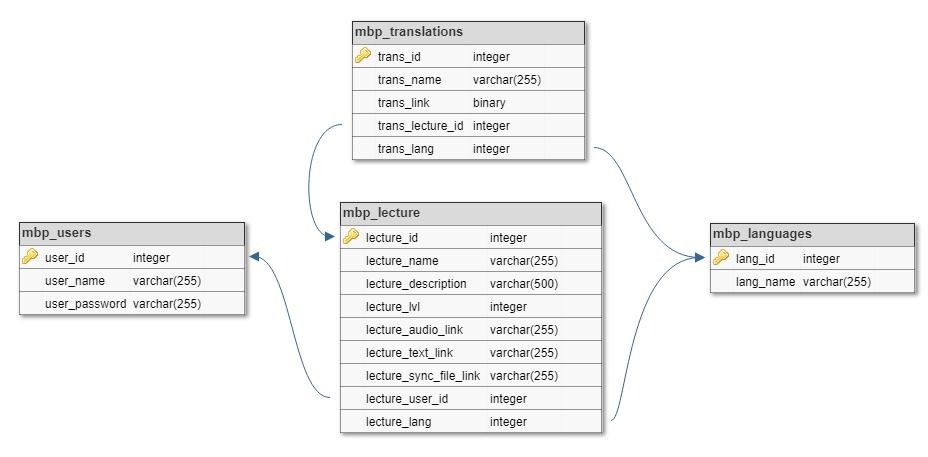
\includegraphics[width=\textwidth]{db_model.jpg}
Zachytáva dátový model databázy online knižnice a registrovaných používateľov.
Tabuľka \textbf{mbp\_users} obsahuje id, prihlasovacie meno a heslo registrovaných užívateľov. 
Tabuľka \textbf{mbp\_translations} obsahuje údaje o dostupných prekladoch textov k jednotlivým lekciám. Obsahuje id, názov, link, id lekcie ku ktorej patrí a id jazyka, v ktorom preklad je.
Tabuľka \textbf{mbp\_languages} je tabuľka jazykov, ktoré aplikácia ponúka, t.j tie jazyky, ktorých náhrávky si môžte vypočuť z online knižnice. Tabuľka obsahuje id a názov jazyka.
Tabuľka \textbf{mbp\_lecture} je tabuľka, ktorá obsahuje údaje k jednotlivým lekciám, t.j obsahuje id, názov, popis, úroveň obtiažnosti, linky k audio, textovému a synchronizačnému súboru, id jazyka danje lekcie a id usera, ktorý pridal lekciu.

\subsection{Formáty súborov}
\subsubsection{Audio súbor}
Súbor môže mať koncovku .wav alebo .mp3. Je rozdelený podľa synchronizačného súboru, a teda je ho možné prehrávať postupne po blokoch alebo náhodne.
\subsubsection{Textový súbor}
Súbor má koncovku .txt a kódovanie v UTF-8, prípadne UTF-8 BOM. Obsahuje text audia, v ktorom sú bloky oddelené znakom "\|".
\subsubsection{Synchronizačný súbor}
Dáta v tomto súbore sú uložené vo formáte json a určujú ako sú rozdelené bloky v audiu. V položke "blocks" sú uložené časové stopy,t.j. časová stopu konca bloku.
V položke "skips" sú zasa uložené bloky, ktoré reč neobsahujú a treba ich preskočiť. Kódovanie tohto súboru je v UTF-8, prípadne UTF-8 BOM. Súbor má koncovku .mbpsf.

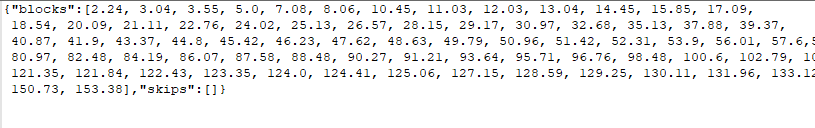
\includegraphics[width=\textwidth]{sync.png}


\subsection{Komunikačné protokoly}
Súbory sa vyberajú z lokálneho disku, na ich výber sa používa ''filePicker'' HTML5 element.

Na čítanie dát zo súboru(textového, synchronizačného) sa využíva js trieda FileReader, ktorá prečíta údaje a pošle ich na ďalšie spracovanie. 
Na spracovanie audio súboru sa používa metóda triedy FileReader - instanceOfFileReader.readAsDataURL(file), ktorá vráti dáta súboru vo formáte base64.
%============================================================
%====   Návrh používateľského rozhrania
%============================================================
\section{Návrh používateľského rozhrania }

\subsection{Edit MediaBlockPlayer SyncFile}
Stránka slúži na vytváranie súborov SyncFile. Používateľ si na začiatku vyberie textový súbor a audio súbor. Taktiež si môže vybrať súbor SyncFile. V tom prípade sa načíta už existujúci súbor a môže sa upravovať, v opačnom prípade sa vytvorí nový súbor SyncFile. Ak má používateľ vybraté všetky položky s ktorými chce pracovať, tlačidlo START EDITING ho presunie na ďalšiu stránku Setting Block ending Time Markers. Ak nechce pokračovať, stačí tlačidlo CANCEL, ktoré ho vráti na domovskú stránku.

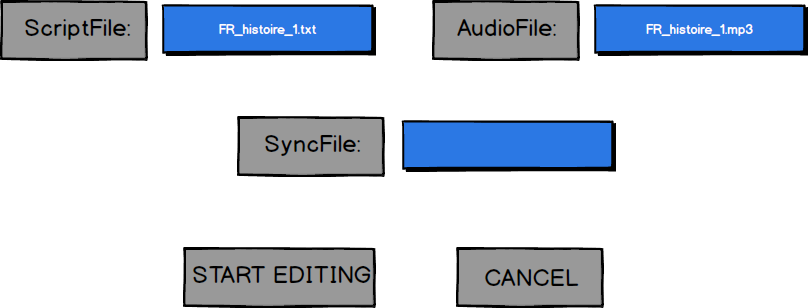
\includegraphics[width=\textwidth]{gui1.png}

\subsection{Setting Block ending Time Markers}
Na stránke Setting Block ending Time Markers pracujeme na vytváraní/editovaní SyncFilu. V okne pod labelom Script sa nachádza text s ktorým pracujeme, pričom aktuálny blok na ktorom sa nachádzame je zvýraznený farbou a podčiarknuté bloky už majú nastavenú časovú značku. Tento text slúži pre používateľa iba na čítanie, v okne samotnom sa nedá upravovať. Časová značka je v texte reprezentovaná ako „|“, a ak je vynechaná nejaká časť audia, tak je označená v texte ako „<SKIPPED>“. Vďaka Buttonom Previous Block/Next Block sa vieme posúvať po blokoch dopredu alebo dozadu. Vpred však vieme ísť iba ak má súčasný blok nastavenú už časovú značku, ktorá zodpovedá koncu bloku.

V sekcií Audio pomocnou Buttonu Play/Pause spúšťame audio nahrávku, sú k dispozícií aj dve tlačidlá +/- na lepšiu prácu s nahrávkou, vďaka ktorým sa vieme posúvať o zadaný interval 0.1s (tento môže používateľ zvýšiť alebo znížiť). Ak sme rozhodnutí nastaviť časovú značku, tak klikneme na tlačidlo OK-Next, ktoré umiestni časovú značku a posunie sa na ďalší blok v texte. Ak chceme pre kontrolu znovu spustiť časť nahrávky k danému bloku, tlačidlo Replay nám prehrá túto časť. Button SKIP Interval nám dovoľuje vynechať časť audio (napríklad ak nesúvisí s textom), opačne funguje button Remove SKIPPED interval vďaka ktorej zrušíme značku SKIPPED a teda časť nahrávky už nebude vynechaná. 

Button EDIT/SPLIT/MERGE Block slúži na spájanie, upravovanie alebo rozdelenie blokov. Po kliknutí na tlačidlo nás presmeruje na ďalšiu stránku EDIT/SPLIT/MERGE Block.

Ak je používateľ s prácou hotový a chce si ju uložiť klikne na button Save+Exit, ktorý ho presunie na okno Save and Exit, ak nechce súbor ukladať stlačí button CANCEL ktorý všetky zmeny zruší a vráti používateľa na domovskú stránku.

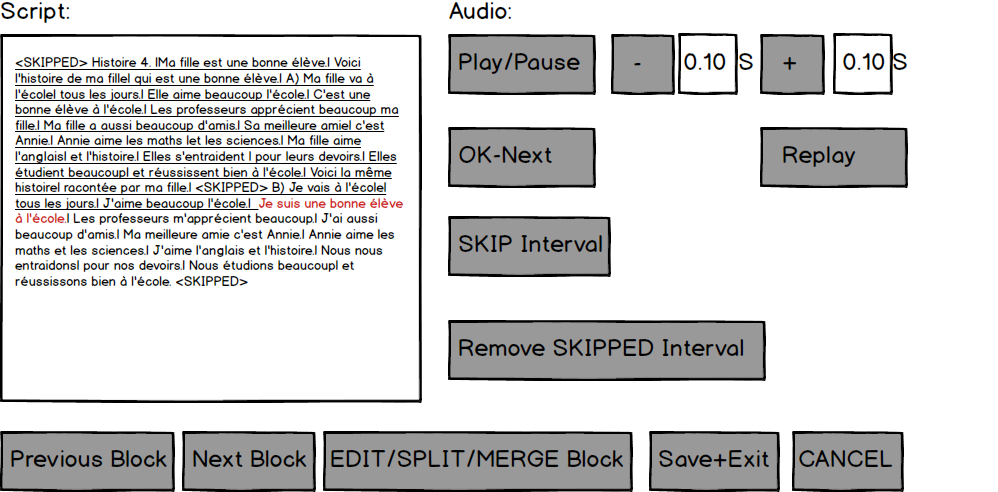
\includegraphics[width=\textwidth]{gui2.png}

\subsection{EDIT/SPLIT/MERGE Block}
V tomto okne si môže používateľ opraviť text aktuálneho bloku, pridať značku do bloku čím ho rozdelí na dva, alebo buttonom Merge with the next block spojiť s nasledujúcim blokom do jedného. Ak so zmenami skončil stlačí tlačidlo Apply edited changes to the Script, ak chce zmeny uložiť natrvalo alebo tlačidlo CANCEL ak chce zmeny zrušiť.

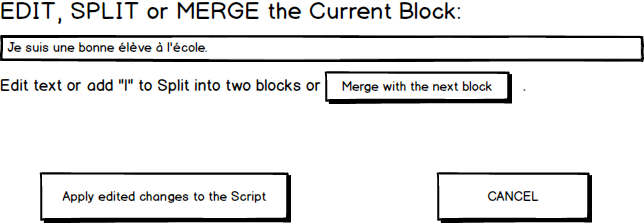
\includegraphics[width=\textwidth]{gui3.png}

\subsection{Save and Exit}
Keď už máme súbor vytvorený, uložíme súbor SyncFile. Vytvoríme názov, default je [AudioFile].mbpsf. A uložíme aj súbor ScriptFile ak bol editovaný. Do Audio súboru nijako nezasahujeme. Kliknutím na Save+Exit sa uložia súbory a vrátime sa na domovskú stránku, pri kliknutí na button Exit without Saving sa vrátime taktiež na domovskú stránku ale súbory sa nám neuložia. Posledný button nás vráti na stránku Setting Block ending Time Markers ak chceme vykonať ešte nejaké zmeny.

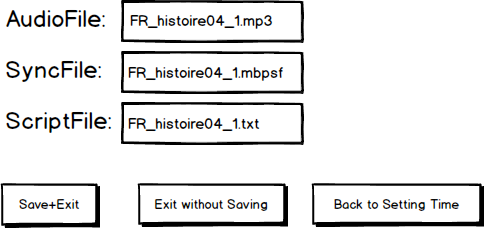
\includegraphics[width=\textwidth]{gui4.png}

%============================================================
%====   Návrh implementácie
%============================================================
\section{Návrh implementácie}

\subsection{GUI interakcia s používateľom}

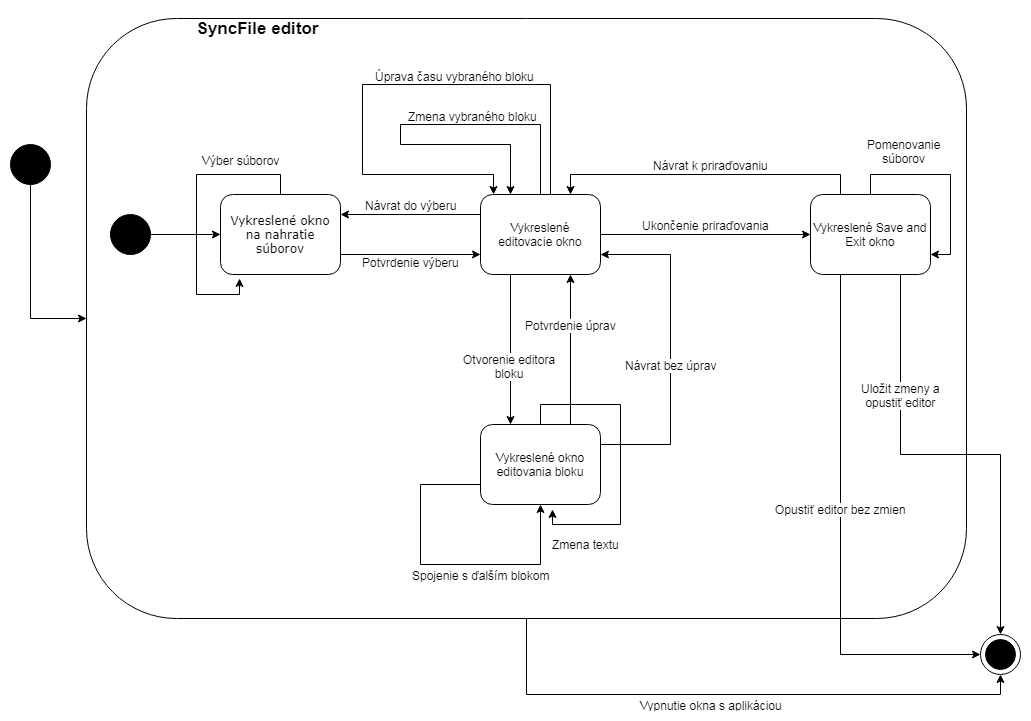
\includegraphics[width=\textwidth]{uml_state.png}

\subsubsection{}
Tento stavový diagram reprezentuje do akých stavov sa môže dostať GUI. 

\subsubsection{}
Diagram modeluje stavy SyncFile editora, ktorý je iba časťou aplikácie.

\subsubsection{}
Začiatok je označený s čiernym plným kruhom, a koncový stav je označený s čiernym plným kruhom s okrajom. 

\subsubsection{}
Prechody medzi stavmi vyvoláva používateľ.

\subsubsection{}
Po vstupe do SyncFile editora bude používateľ vyzvaný k nahratiu súborov z lokálneho disku. 
Po nahraní súborov bude používateľovy umožnené priraďovanie časových značiek k blokom.
Používateľ bude mať možnosť vstúpiť do editora bloku. 
Po opustení editora sa dostane späť k priraďovaniu časových značiek blokom.
Následne používateľ dostane možnosť edivované súbory stiahnuť a SyncFile editor ukončiť.

\subsection{Triedy aplikácie}

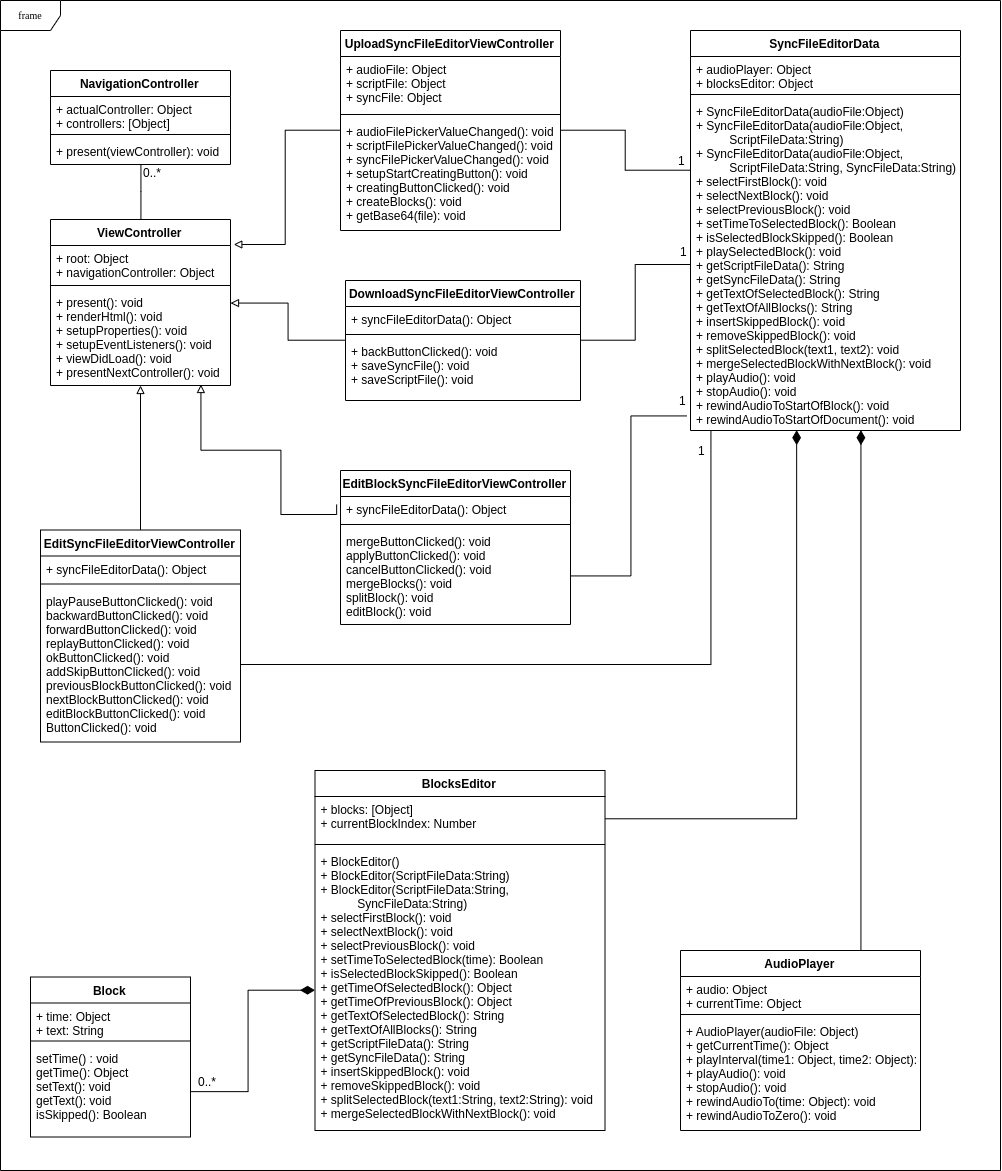
\includegraphics[width=\textwidth]{uml_class.png}

\subsubsection{}
NavigationController drží v pamäti práve ktorý screen aplikácie treba vyrenderovať.

\subsubsection{}
Jednotlivé screeny predstavujú triedy odvodené od ViewController.
Každá podtrieda má svoje funkcie aby splnil požiadavky čo na danom screen-e treba vykonať.

\subsubsection{}
Trieda Block udržuje parametre jedného bloku - čas konca bloku a text bloku.
V prípade, že text bloku nieje definovaný, tak daný blok predstavuje skipped interval.

\subsubsection{}
Trieda BlocksEditor udržuje dáta o všetkých blokoch. Trieda vie editovať bloky, zmeniť označený blok, pridávať a odoberať bloky, vygenerovať SyncFile a ScriptFile.

\subsubsection{}
Trieda AudioPlayer umožnuje prácu s audio nahrávkou.

\subsubsection{}
Trieda SyncFileEditorData zoskupuje media block dáta s ktorými SyncFile editor pracuje.

\subsection{Komponenty aplikácie}

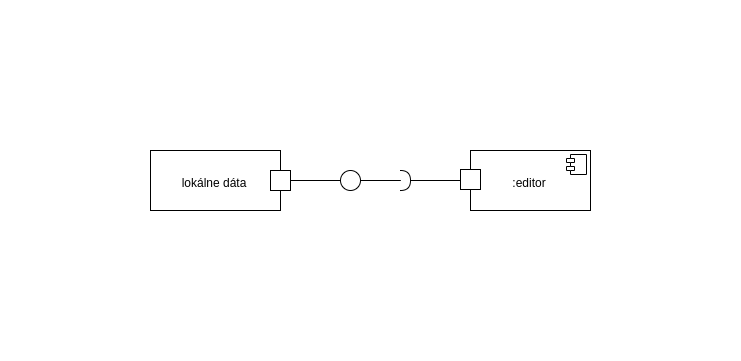
\includegraphics[width=\textwidth]{uml_component.png}

\subsubsection{}
SyncFile editor pozostáva z jednej komponenty nazvanej editor, ktorá pracuje s lokálnymi dátami.

\end{document}
